\documentclass[8pt]{article}
\RequirePackage{amsmath}
\RequirePackage{bytefield}
\RequirePackage{graphicx}
\RequirePackage{newtxmath}

\setlength{\oddsidemargin}{-0.25in} % Left margin of 1 in + 0 in = 1 in
\setlength{\textwidth}{7in}   % Right margin of 8.5 in - 1 in - 6.5 in = 1 in
\setlength{\topmargin}{-.75in}  % Top margin of 2 in -0.75 in = 1 in
\setlength{\textheight}{9.2in}  % Lower margin of 11 in - 9 in - 1 in = 1 in

\mathchardef\mhyphen="2D

% terminology

\newcommand{\Zcash}{\textbf{Zcash} }
\newcommand{\Zerocash}{\textbf{Zerocash} }
%
% key pairs:
\newcommand{\PublicAddress}{\mathsf{addr_{pk}}}
\newcommand{\PrivateAddress}{\mathsf{addr_{sk}}}
\newcommand{\PublicAddressName}{\emph{protected address}}
\newcommand{\PrivateAddressName}{\emph{protected address secret}}
\newcommand{\PublicAddressLeadByte}{\mathbf{0x92}}
\newcommand{\PrivateAddressLeadByte}{\mathbf{0x93}}
\newcommand{\SpendAuthorityPublic}{\mathsf{a_{pk}}}
\newcommand{\SpendAuthorityPrivate}{\mathsf{a_{sk}}}
\newcommand{\SpendAuthorityName}{\emph{spend authority}}
\newcommand{\TransmitPublic}{\mathsf{pk_{enc}}}
\newcommand{\TransmitPrivate}{\mathsf{sk_{enc}}}
\newcommand{\TransmitPublicName}{\emph{key-private encryption}}
\newcommand{\TransmitPrivateName}{\emph{key-private decryption}}
\newcommand{\Value}{\mathsf{v}}
%
% buckets
\newcommand{\Bucket}{\mathsf{b}}
\newcommand{\BucketRand}{\mathsf{r}}
\newcommand{\BucketAddressRand}{\mathsf{\uprho}}
\newcommand{\BucketPlaintextName}{\emph{transmitted bucket plaintext}}
\newcommand{\BucketCiphertextName}{\emph{transmitted bucket ciphertext}}
\newcommand{\BucketCommitmentName}{\emph{bucket commitment}}
\newcommand{\BucketPlaintextVersionByte}{\mathbf{0x00}}
\newcommand{\CRH}{\mathbf{CRH}}
\newcommand{\PRF}[2]{\mathbf{PRF_{#1}^{#2}}}
\newcommand{\PRFaddr}[1]{\PRF{#1}{addr}}
\newcommand{\PRFsn}[1]{\PRF{#1}{sn}}
\newcommand{\PRFpk}[2]{\PRF{#1}{pk_{#2}}}
\newcommand{\SHA}{\mathtt{SHA256Compress}}
\newcommand{\SHAName}{\emph{SHA-256 compression}}
\newcommand{\SHAOrig}{\emph{SHA-256}}
\newcommand{\bm}{\mathbf{\mathtt{bm}}}
\newcommand{\InternalHashK}{\mathsf{k}}
\newcommand{\InternalHash}{\mathsf{InternalH}}
% merkle tree
\newcommand{\MerkleDepth}{\mathsf{d}}
\newcommand{\PourTx}{\mathtt{PourTx}}
\newcommand{\sn}{\mathsf{sn}}
% bitcoin
\newcommand{\vin}{\mathtt{vin}}
\newcommand{\vout}{\mathtt{vout}}
\newcommand{\vpour}{\mathtt{vpour}}
\newcommand{\vpubOld}{\mathtt{vpub\_old}}
\newcommand{\vpubNew}{\mathtt{vpub\_new}}
\newcommand{\anchor}{\mathtt{anchor}}
\newcommand{\scriptSig}{\mathtt{scriptSig}}
\newcommand{\scriptPubKey}{\mathtt{scriptPubKey}}
\newcommand{\serials}{\mathtt{serials}}
\newcommand{\commitments}{\mathtt{commitments}}
\newcommand{\bucketCiphertexts}{\mathtt{bucketCiphertexts}}
\newcommand{\rt}{\mathsf{rt}}
% pour
\newcommand{\hSig}{\mathsf{h_{Sig}}}
\newcommand{\Nold}{N_{Old}}
\newcommand{\Nnew}{N_{New}}
\newcommand{\vmacs}{\mathtt{vmacs}}
\newcommand{\zkproof}{\mathtt{zkproof}}
\newcommand{\PourStatement}{\texttt{POUR}}
\newcommand{\PourProof}{\pi_{\PourStatement}}
\newcommand{\vpubold}{\mathsf{vpub_{old}}}
\newcommand{\vpubnew}{\mathsf{vpub_{new}}}
\newcommand{\bOld}[1]{\mathsf{b_{#1}^{old}}}
\newcommand{\bNew}[1]{\mathsf{b_{#1}^{new}}}
\newcommand{\vOld}[1]{\mathsf{v_{#1}^{old}}}
\newcommand{\vNew}[1]{\mathsf{v_{#1}^{new}}}
\newcommand{\NP}{\mathsf{NP}}
\newcommand{\path}[1]{\mathsf{path_{#1}}}

% TODO: COMM is used in the zerocash paper. We should use it
% where applicable. (The paper treats bm as a COMM, when it really
% isn't anymore after changes made by the academics that weren't
% included in the paper).
%\newcommand{\COMM}[1]{\mathbf{COMM_{#1}}}

%eli macros
\usepackage{color}
\newcommand{\eli}[1]{{\color{magenta}\sf{Eli: #1}}}
\newcommand{\sean}[1]{{\color{blue}\sf{Sean: #1}}}
\newcommand{\taylor}[1]{{\color{red}\sf{Taylor: #1}}}
\newcommand{\daira}[1]{{\color{green}\sf{Daira: #1}}}


\newcommand{\BucketCommitment}[1]{\mathtt{BucketCommitment(#1)}}


\begin{document}

\title{Zcash Protocol Specification}
\author{Sean Bowe | Daira Hopwood | Taylor Hornby}
\date{\today}
\maketitle
\section{Introduction}

\Zcash is an implementation of the \emph{decentralized anonymous payment} (DAP) scheme \Zerocash with minor adjustments to terminology, functionality and performance. It bridges the existing value transfer scheme used by Bitcoin with an anonymous payment scheme protected by zero-knowledge succinct non-interactive arguments of knowledge (\textbf{zk-SNARK}s). \sean{I want to make sure we add citations here for the original paper}

\section{Concepts}

\subsection{Integers and Endianness}

Abstractly, integers have a signedness (signed or unsigned), and a bit length.
The limits are the same as for the usual two's complement system. All integers
in the publicly-visible \Zcash protocol are encoded in big endian two's
complement.

If unspecified, curve points, field elements, etc., are encoded according to the
crypto libraries the \Zcash implementation uses.

\subsection{Cryptographic Functions}

\subparagraph{}

$\CRH$ is a collision-resistant hash function. In \Zcash, the $\SHAName$ function is used which takes a 512-bit block and produces a 256-bit hash. This is different from the $\SHAOrig$ function, which hashes arbitrary-length strings.

\subparagraph{}

$\PRF{x}{}$ is a pseudo-random function seeded by $x$. Three \textit{independent} $\PRF{x}{}$ are needed in our scheme: $\PRFaddr{x}$, $\PRFsn{x}$, and $\PRFpk{x}{i}$. It is required that $\PRFsn{x}$ be collision-resistant. In \Zcash, the $\SHAName$ function is used to seed all three of these functions. The bits $\mathtt{00}$, $\mathtt{01}$ and $\mathtt{10}$ are included (respectively) within the blocks that are hashed, ensuring that the functions are independent.

\begin{equation*}
\SpendAuthorityPublic = \PRFaddr{\SpendAuthorityPrivate}(0) = \CRH\left(
\;
\begin{bytefield}[bitwidth=0.07em]{512}
	\bitbox{242}{256 bit $\SpendAuthorityPrivate$} &
	\bitbox{14}{0} &
	\bitbox{14}{0} &
	\bitbox{242}{$0^{254}$} &
\end{bytefield}
\enspace
\right)
\end{equation*}

\begin{equation*}
\sn = \PRFsn{\SpendAuthorityPrivate}(\BucketAddressRand) = \CRH\left(
\;
\begin{bytefield}[bitwidth=0.07em]{512}
	\bitbox{242}{256 bit $\SpendAuthorityPrivate$} &
	\bitbox{14}{0} &
	\bitbox{14}{1} &
	\bitbox{242}{254 bit truncated $\BucketAddressRand$} &
\end{bytefield}
\enspace
\right)
\end{equation*}


\begin{equation*}
h_i = \PRFpk{\SpendAuthorityPrivate}{i}(\hSig) = \CRH\left(
\;
\begin{bytefield}[bitwidth=0.07em]{512}
	\bitbox{242}{256 bit $\SpendAuthorityPrivate$} &
	\bitbox{14}{1} &
	\bitbox{14}{0} &
	\bitbox{14}{i} &
	\bitbox{241}{253 bit truncated $\hSig$}
\end{bytefield}
\enspace
\right)
\end{equation*}

\subsection{Confidential Address Key Pair}

\subparagraph{}

A key pair $(\PublicAddress, \PrivateAddress)$ is generated by users who wish to receive coins under this scheme. The public $\PublicAddress$ is called a $\PublicAddressName$ and is a tuple $(\SpendAuthorityPublic, \TransmitPublic)$ which are the public components of a $\SpendAuthorityName$ key pair $(\SpendAuthorityPublic, \SpendAuthorityPrivate)$ and a $\TransmitPublicName$ key pair $(\TransmitPublic, \TransmitPrivate)$. The private $\PrivateAddress$ is called a $\PrivateAddressName$ and is a tuple $(\SpendAuthorityPrivate, \TransmitPrivate)$ which are the respective \textit{private} components of the aforementioned $\SpendAuthorityName$ and $\TransmitPublicName$ key pairs.

\subparagraph{}

Although users can accept payment from multiple parties with a single $\PublicAddress$ without either party being aware, it is still recommended to generate a new address for each expected transaction to maximize privacy in the event that multiple sending parties are compromised or collude.

\subsection{Buckets}

\subparagraph{}

A bucket (denoted $\Bucket$) is a tuple $(\Value, \SpendAuthorityPublic, \BucketRand, \BucketAddressRand)$ which represents that a value $\Value$ is spendable by the recipient who holds the $\SpendAuthorityName$ key pair $(\SpendAuthorityPublic, \SpendAuthorityPrivate)$ such that $\SpendAuthorityPublic=\PRFaddr{\SpendAuthorityPrivate}(0)$. $\BucketRand$ and $\BucketAddressRand$ are randomly generated tokens by the sender. Only a hash of these values is disclosed publicly, which allows these random tokens to blind the value and recipient \textit{except} to those who possess these tokens.

\subparagraph{In-band secret distribution}

In order to send the secret $\Value$, $\BucketRand$ and $\BucketAddressRand$ to the recipient (necessary for the recipient to later spend) \textit{without} requiring an out-of-band communication channel, the $\TransmitPublicName$ public key $\TransmitPublic$ is used to encrypt these secrets to form an \BucketCiphertextName. The recipient's possession of the associated $(\PublicAddress, \PrivateAddress)$ (which contains both $\SpendAuthorityPublic$ and $\TransmitPrivate$) is used to reconstruct the original bucket.

\subparagraph{Bucket commitments}

The underlying $\Value$ and $\SpendAuthorityPublic$ are blinded with $\BucketRand$ and $\BucketAddressRand$ using the collision-resistant hash function $\CRH$ in a multi-layered process. The resulting hash $\bm = \BucketCommitment{\Bucket}$.

% TODO: this appears to be ineffective
\begin{flushright}

\begin{equation*}
\InternalHash := \CRH\left(
\;
\begin{bytefield}[bitwidth=0.07em]{512}
	\bitbox{256}{256 bit $\SpendAuthorityPublic$} &
	\bitbox{256}{256 bit $\BucketAddressRand$}
\end{bytefield}
\enspace
\right)
\end{equation*}

\begin{equation*}
\InternalHashK := \CRH\left(
\;
\begin{bytefield}[bitwidth=0.07em]{512}
	\bitbox{256}{256 bit $\BucketRand$} &
	\bitbox{256}{256 bit $\InternalHash$}
\end{bytefield}
\enspace
\right)
\end{equation*}

\begin{equation*}
\bm := \CRH\left(
\;
\begin{bytefield}[bitwidth=0.07em]{512}
	\bitbox{64}{64 bit $\Value$} &
	\bitbox{192}{192 bit padding} &
	\bitbox{256}{256 bit $\InternalHashK$}
\end{bytefield}
\enspace
\right)
\end{equation*}

\end{flushright}

\subparagraph{Serials}

A serial number (denoted $\sn$) equals $\PRFsn{\SpendAuthorityPrivate}(\BucketAddressRand)$. Buckets are spent by proving knowledge of $\BucketAddressRand$ and $\SpendAuthorityPrivate$ in zero-knowledge while disclosing $\sn$, allowing $\sn$ to be used to prevent double-spending.

\subsection{Bucket Commitment Tree}

\begin{center}
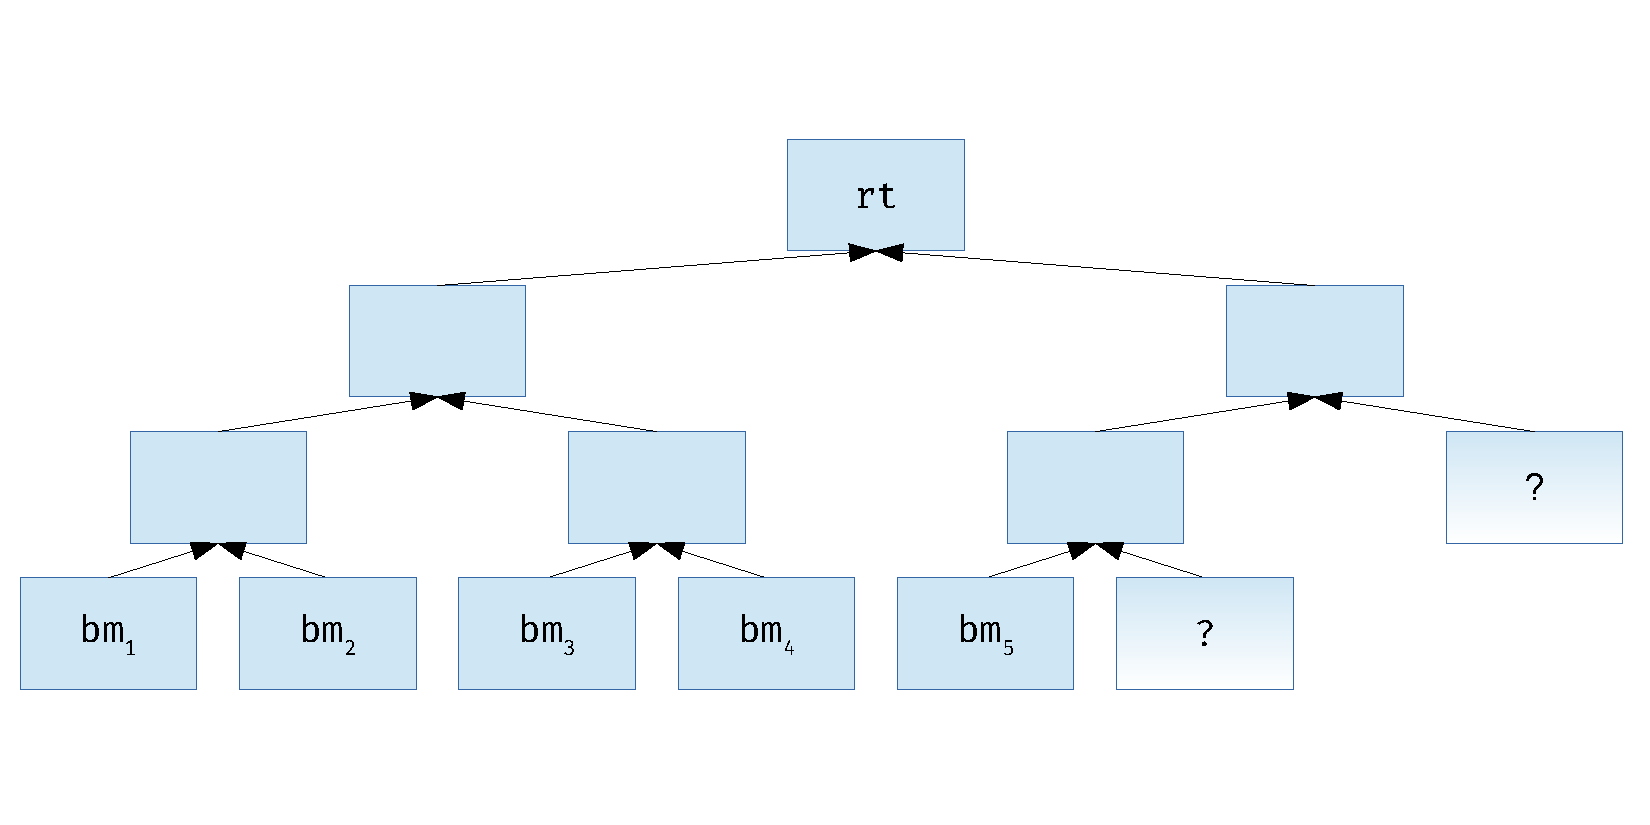
\includegraphics[scale=.4]{incremental_merkle}
\end{center}

\subparagraph{}

The bucket commitment tree is an \textit{incremental merkle tree} of depth $\MerkleDepth$ used to store bucket commitments that transactions produce. Just as the \textit{unspent transaction output set} (UTXO) used in Bitcoin proper, it is used to express the existence of value and the capability to spend it. However, unlike the UTXO, it is \textit{not} the job of this tree to protect against double-spending, as it is append-only.

\subparagraph{}

Blocks in the blockchain are associated (by all nodes) with the root of this tree after all of its constituent transactions' bucket commitments have been entered into the tree associated with the previous block.

\subsection{Spent Serials Map}

\subparagraph{}
\eli{Would be good to formally define the structure of a transaction, similar to the way a bucket is defined (as a quadruple).}
Transactions insert \eli{a tx is just a string, so it doesn't insert anything. Rather, nodes process tx's and the ``good'' ones lead to the addition of serials to the spent serials map.} serials into a \textit{spent serials map} which is maintained alongside the UTXO by all nodes. Transactions that attempt to insert a serial into this map that already exists within it are invalid as they are attempting to double-spend. \eli{After defining \emph{transaction}, one should define what a \emph{legal tx} is (this definition depends on a particular blockchain) and only then can one talk about ``attempts'' of transactions, and insertions of serial numbers into the spent serials map.}

\subsection{Bitcoin Transactions}

\subparagraph{}
\eli{Please formally define what a tx is. I don't think it's merely a sequence of inputs and outputs. The outputs are probably buckets (as defined above) and maybe the inputs are, too. Perhaps one should talk about a tx-bucket (which is unhidden) and a tx which is mostly hashed-stuff + a SNARK)}
Bitcoin transactions consist of a vector \eli{sequence? vector implies ``vector space'' which doens't exist here} of inputs ($\mathtt{vin}$) and a vector of outputs ($\mathtt{vout}$). Inputs and outputs are associated with a value \eli{assuing a tx-bucket is a pair of sequences --- an input-sequence and an output-sequence, and each sequence is a sequence of buckets, one should define the in-value of the tx-bucket as the sum of values in the in-buckets (ditto for out-value) and the remaining value is their difference}. The total value of the outputs must not exceed the total value of the inputs.

\subparagraph{Value pool}

Transaction inputs insert value into a \textit{value pool}, and transaction outputs remove value from this pool. The remaining value in the pool is available to miners as a fee.

\section{Pour Transactions ($\PourTx$)}

\eli{Hmm, I think things are starting to get confused here, let's try to clarify the theory/crypto. Informally, buckets and transactions are \emph{data}, whereas Pour is best thought of as a \emph{circuit} that outputs either $1$ (``true'') or $0$ (``false''). The theory of SNARKs (as supported by libsnark) is such that if the circuit outputs ``true'' then you can generate a SNARK for that set of inputs, and otherwise you can't (its cryptographically infeasible to do so). So we should describe formally what the \emph{inputs} to the Pour circuit are, and then define the \emph{computation preformed} by the Pour circuit, i.e., describe how it decides whether to output $0$ or $1$. More below}
\subparagraph{}

$\PourTx$s are the primary operations \eli{In the academic paper, a Pour is a circuit (that defines an NP-language), and that circuit is the most crucial part of the construction. So if you want to use ``Pour'' to describe the algorithm that generates a tx, you'll be (i) deviating from the academic paper in a rather confusing way and (ii) you still need to define the ``Pour-circuit'' which is at the heart of the construction} performed by transactions that interact with our scheme. In principle, it is the action of spending $\Nold$ buckets $\bOld{}$ and creating $\Nnew$ buckets $\bNew{}$. \Zcash transactions have an additional field $\vpour$, which is a vector of $\PourTx$s. Each $\PourTx$ consists of:
\eli{reached here}
\begin{list}{}{}

\item $\vpubOld$ which is a value $\vpubold$ that the pour removes from the value pool.

\item $\vpubNew$ which is a value $\vpubnew$ that the pour inserts into the value pool.

\item $\anchor$ which is a merkle root $\rt$ of the bucket commitment tree at some block height in the past, or the merkle root produced by a previous pour in this transaction. \sean{We need to be more specific here.}

\item $\scriptSig$ which is a Bitcoin script which creates conditions for acceptance of a $\PourTx$ in a transaction. The $\SHA$ hash of this value is $\hSig$.

\item $\scriptPubKey$ which is a Bitcoin script used to satisfy the conditions of the $\scriptSig$.

\item $\serials$ which is an $\Nold$ size vector of serials $\sn^{old}_{1}, \sn^{old}_{2}, ..., \sn^{old}_{\Nold}$.

\item $\commitments$ which is a $\Nnew$ size vector of bucket commitments $\bm^{new}_{1}, \bm^{new}_{2}, ..., \bm^{new}_{\Nnew}$.

\item $\bucketCiphertexts$ which is a $\Nnew$ size vector each element of which is a \BucketCiphertextName.

\item $\vmacs$ which is a $\Nold$ size vector of message authentication codes $h$ which bind $\hSig$ to each $\SpendAuthorityPrivate$ of the $\PourTx$.

\item $\zkproof$ which is the zero-knowledge proof $\PourProof$.

\end{list}

\subparagraph{Merkle root validity}

A $\PourTx$ is valid if $\rt$ is a bucket commitment tree root found in either the blockchain or a merkle root produced by inserting the bucket commitments of a previous $\PourTx$ in the transaction to the bucket commitment tree identified by that previous $\PourTx$'s $\anchor$.

\subparagraph{Non-malleability}

A $\PourTx$ is valid if the script formed by appending $\scriptPubKey$ to $\scriptSig$ returns $true$. The $\scriptSig$ is cryptographically bound to $\PourProof$.

\subparagraph{Balance}

A $\PourTx$ can be seen, from the perspective of the transaction, as an input and an output simultaneously. $\vpubOld$ takes value from the value pool and $\vpubNew$ adds value to the value pool. As a result, $\vpubOld$ is treated like an \textit{output} value, whereas $\vpubNew$ is treated like an \textit{input} value.

\subparagraph{Commitments and Serials}

Transactions which contain $\PourTx$s, when entered into the blockchain, append to the bucket commitment tree with all constituent bucket commitments. All of the constituent serials are also entered into the spent serials map of the blockchain \textit{and} mempool. Transactions are not valid if they attempt to add a serial to the spent serials map that already exists.

\subsection{$\PourProof$}

\subparagraph{}

In \Zcash, $\Nold$ and $\Nnew$ are both $2$.

\subparagraph{}

A valid instance of $\PourProof$ assures that given a \textit{primary input} ($\rt$, $\sn^{old}_{1}$, $\sn^{old}_{2}$, $\bm^{new}_{1}$, $\bm^{new}_{2}$, $\vpubold$, $\vpubnew$, $\hSig$, $h_1$, $h_2$), a witness of \textit{auxiliary input} ($\path{1}$, $\path{2}$, $\bOld{1}$, $\bOld{2}$, $\SpendAuthorityPrivate^{old}_1$, $\SpendAuthorityPrivate^{old}_2$, $\bNew{1}$, $\bNew{2}$) exists, where:

\begin{list}{}{}

\item for each $i \in \{1, 2\}$: $\bOld{i}$ = $(\vOld{i}, \SpendAuthorityPublic^{old}_i, \BucketRand^{old}_i, \BucketAddressRand^{old}_i)$

\item for each $i \in \{1, 2\}$: $\bNew{i}$ = $(\vNew{i}, \SpendAuthorityPublic^{new}_i, \BucketRand^{new}_i, \BucketAddressRand^{new}_i)$.

\item The following conditions hold:

\end{list}

\subparagraph{Merkle path validity}

for each $i \in \{1, 2\}$ $\mid$ $\vOld{i} \neq 0$: $\path{i}$ must be a valid path of depth $\MerkleDepth$ from \linebreak $\BucketCommitment{\bOld{i}}$ to bucket commitment merkle tree root $\rt$.

\subparagraph{Balance}

$\vpubold + \vOld{1} + \vOld{2} = \vpubnew + \vNew{1} + \vNew{2}$.

\subparagraph{Serial integrity}

for each $i \in \{1, 2\}$: $\PRFsn{\SpendAuthorityPrivate^{old}_{i}}(\BucketAddressRand^{old}_{i})$ = $\sn^{old}_{i}$.

\subparagraph{Spend authority}

for each $i \in \{1, 2\}$: $\SpendAuthorityPublic^{old}_{i}$ = $\PRFaddr{\SpendAuthorityPrivate^{old}_{i}}(0)$.

\subparagraph{Non-malleability}

% TODO: protocol is really gross here, let's clarify the
% indices and use of PRFpk independence from other h sdfhjgahsdjkgfas
for each $i \in \{1, 2\}$: $h_i$ = $\PRFpk{\SpendAuthorityPrivate^{old}_i}{i-1}(\hSig)$

\subparagraph{Commitment integrity}

for each $i \in \{1, 2\}$: $\bm^{new}_i$ = $\BucketCommitment{\bNew{i}}$

\section{Encoding addresses, private keys, buckets, and pours}

This section describes how \Zcash encodes public addresses, private keys,
buckets, and pours.

Addresses, keys, and buckets, can be encoded as a byte string; this is called
the \emph{raw encoding}. This byte string can then be further encoded using
Base58Check. The Base58Check layer is the same as for upstream Bitcoin
addresses.

SHA-256 compression function outputs are always represented as strings of 32
bytes.

The language consisting of the following encoding possibilities is prefix-free.

\subsection{Cleartext Public Addresses}

TBD. Identical to Bitcoin?

\subsection{Cleartext Private Keys}

TBD. Identical to Bitcoin?

\subsection{Protected Public Addresses}

A protected address consists of $\SpendAuthorityPublic$ and $\TransmitPublic$.
$\SpendAuthorityPublic$ is a SHA-256 compression function output.
$\TransmitPublic$ is an encryption public key (currently ECIES, but this may
change to Curve25519/crypto\_box), which represents an equivalence class of
two points sharing an $x$ coordinate on an elliptic curve.

\subsubsection{Raw Encoding}

The raw encoding of a protected address consists of:

\begin{equation*}
\begin{bytefield}[bitwidth=0.07em]{520}
	\bitbox{80}{$\PublicAddressLeadByte$} &
    \bitbox{256}{$\SpendAuthorityPublic$ (32 bytes)} &
    \bitbox{256}{A 33-byte encoding of $\TransmitPublic$}
\end{bytefield}
\end{equation*}

\begin{itemize}
    \item A byte, $\PublicAddressLeadByte$, indicating this version of the
        raw encoding of a \Zcash public address.
    \item 32 bytes specifying $\SpendAuthorityPublic$.
    \item An encoding of $\TransmitPublic$: The byte $\mathbf{0x01}$, followed by 32 bytes
        representing the $x$ coordinate of an elliptic curve point according to
        the $\mathsf{FE2OSP}$ primitive specified in section 5.5.4 of IEEE Std 1363-2000.
        [Non-normative note: Since the curve is over a prime field, this is just
            the 32-byte big-endian representation of the $x$ coordinate. The
            overall encoding matches the $\mathsf{EC2OSP{\mhyphen}X}$ primitive
            specified in section 5.5.6.3 of IEEE Std 1363a-2004. It does not
            matter which of the two points with the same $x$ coordinate is used.]
\end{itemize}

\textbf{TODO: check that this lead byte is distinct from other Bitcoin stuff,
and produces `z' as the Base58Check leading character.}

\textbf{TODO: what about the network version byte?}

\textbf{TODO: add bibliographic references for the IEEE standards.}

\subsection{Protected Address Secrets}

A protected address secret consists of $\SpendAuthorityPrivate$ and
$\TransmitPrivate$. $\SpendAuthorityPrivate$ is a SHA-256 compression function
output. $\TransmitPrivate$ is an encryption private key (currently ECIES), which
is an integer.

\subsubsection{Raw Encoding}

The raw encoding of a protected address secret consists of, in order:

\begin{equation*}
\begin{bytefield}[bitwidth=0.07em]{520}
	\bitbox{80}{$\PrivateAddressLeadByte$} &
    \bitbox{256}{$\SpendAuthorityPrivate$ (32 bytes)} &
    \bitbox{256}{$\TransmitPrivate$ (32 bytes)}
\end{bytefield}
\end{equation*}

\begin{itemize}
    \item A byte $\PrivateAddressLeadByte$ indicating this version of the
        raw encoding of a \Zcash private key.
    \item 32 bytes specifying $\SpendAuthorityPrivate$.
    \item 32 bytes specifying a big-endian encoding of $\TransmitPrivate$.
\end{itemize}

\textbf{TODO: check that this lead byte is distinct from other Bitcoin stuff,
and produces `z' as the Base58Check leading character.}

\textbf{TODO: what about the network version byte?}

\subsection{Buckets}

Transmitted buckets are stored on the blockchain in encrypted form, together with
a \BucketCommitmentName $\bm$.

A \BucketCiphertextName is an ECIES key-private encryption of a \BucketPlaintextName
to a \TransmitPublicName key $\TransmitPublic$.

A \BucketPlaintextName consists of $(\Value, \BucketAddressRand, \BucketRand)$, where:

\begin{itemize}
    \item $\Value$ is a 64-bit unsigned integer representing the value of the
        bucket in zatoshi.
    \item $\BucketAddressRand$ is a 32-byte $\PRFsn{\SpendAuthorityPrivate}$ seed.
    \item $\BucketRand$ is a 32-byte COMM trapdoor.
\end{itemize}

Note that the value $s$ described as being part of a bucket/coin in the Zerocash
paper is not encoded because it is fixed to zero.

\subsection{Raw Encoding}

The raw encoding of a \BucketPlaintextName consists of, in order:

\begin{equation*}
\begin{bytefield}[bitwidth=0.05em]{200}
	\bitbox{80}{$\BucketPlaintextVersionByte$} &
    \bitbox{230}{$\Value$ (8 bytes, big endian)} &
    \bitbox{230}{$\BucketAddressRand$ (32 bytes)} &
    \bitbox{230}{$\BucketRand$ (32 bytes)} &
\end{bytefield}
\end{equation*}

\begin{itemize}
    \item A byte $\BucketPlaintextVersionByte$ indicating this version of the raw encoding of a \BucketPlaintextName.
    \item 8 bytes specifying a big-endian encoding of $\Value$.
    \item 32 bytes specifying $\BucketAddressRand$.
    \item 32 bytes specifying $\BucketRand$.
\end{itemize}

\section{Pours (within a transaction on the blockchain)}

TBD.

\section{Transactions}

TBD.

\end{document}
